\documentclass{standalone}
\usepackage{tikz}

\begin{document}

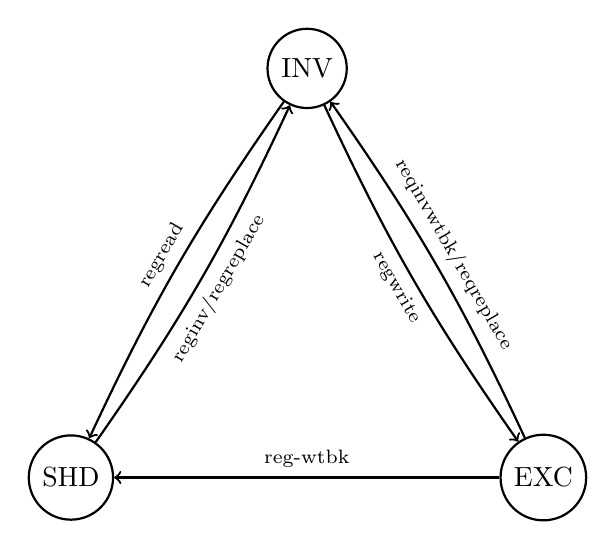
\begin{tikzpicture}[thick]
  \node[draw, circle] (inv) {INV};
  \node[draw, circle, xshift=-3cm, yshift=-5.196cm] (shd) {SHD};
  \node[draw, circle, right of=shd, node distance=6cm] (exc) {EXC};

  \path[->, every node/.style={sloped,anchor=center,above,font=\scriptsize}]
    (inv) edge [bend right=5] node[] {regread} (shd)
    (inv) edge [bend right=5] node[below] {regwrite}  (exc)
    (shd) edge [bend right=5] node[below] {reginv/regreplace}  (inv)

    (exc) edge [bend right=5] node[] {reqinvwtbk/reqreplace}  (inv)
    (exc) edge node[] {reg-wtbk}  (shd);
\end{tikzpicture}

\end{document}

